\section{Statistical Estimation Theory}
\label{sec:SDT}

Once we have faced some of the main concepts involved in estimation problems, we are ready to formalize the problem for a general case.

\subsection{General view of the estimation problem}
\label{subsec:hypotheses_problems}

The design of an estimator consists of constructing a real function that, from the value of certain observation variables, provides predictions about an objective variable (or vector). 

For a general case, we will denote that random variable to be estimated as $S$ which can take any real value. As indicated in Fig. \ref{fig:est_overview}, we assume also that we have access to an observation vector $\bf x$ that can be considered as the realization of a random variable $\bf X$ lying in observation space $\cal X$. Note also that for the estimation task of $s$ or $S$ from $\bf X$ to make sense, there must be some statistical relationship between them.

\begin{figure}
\begin{center}
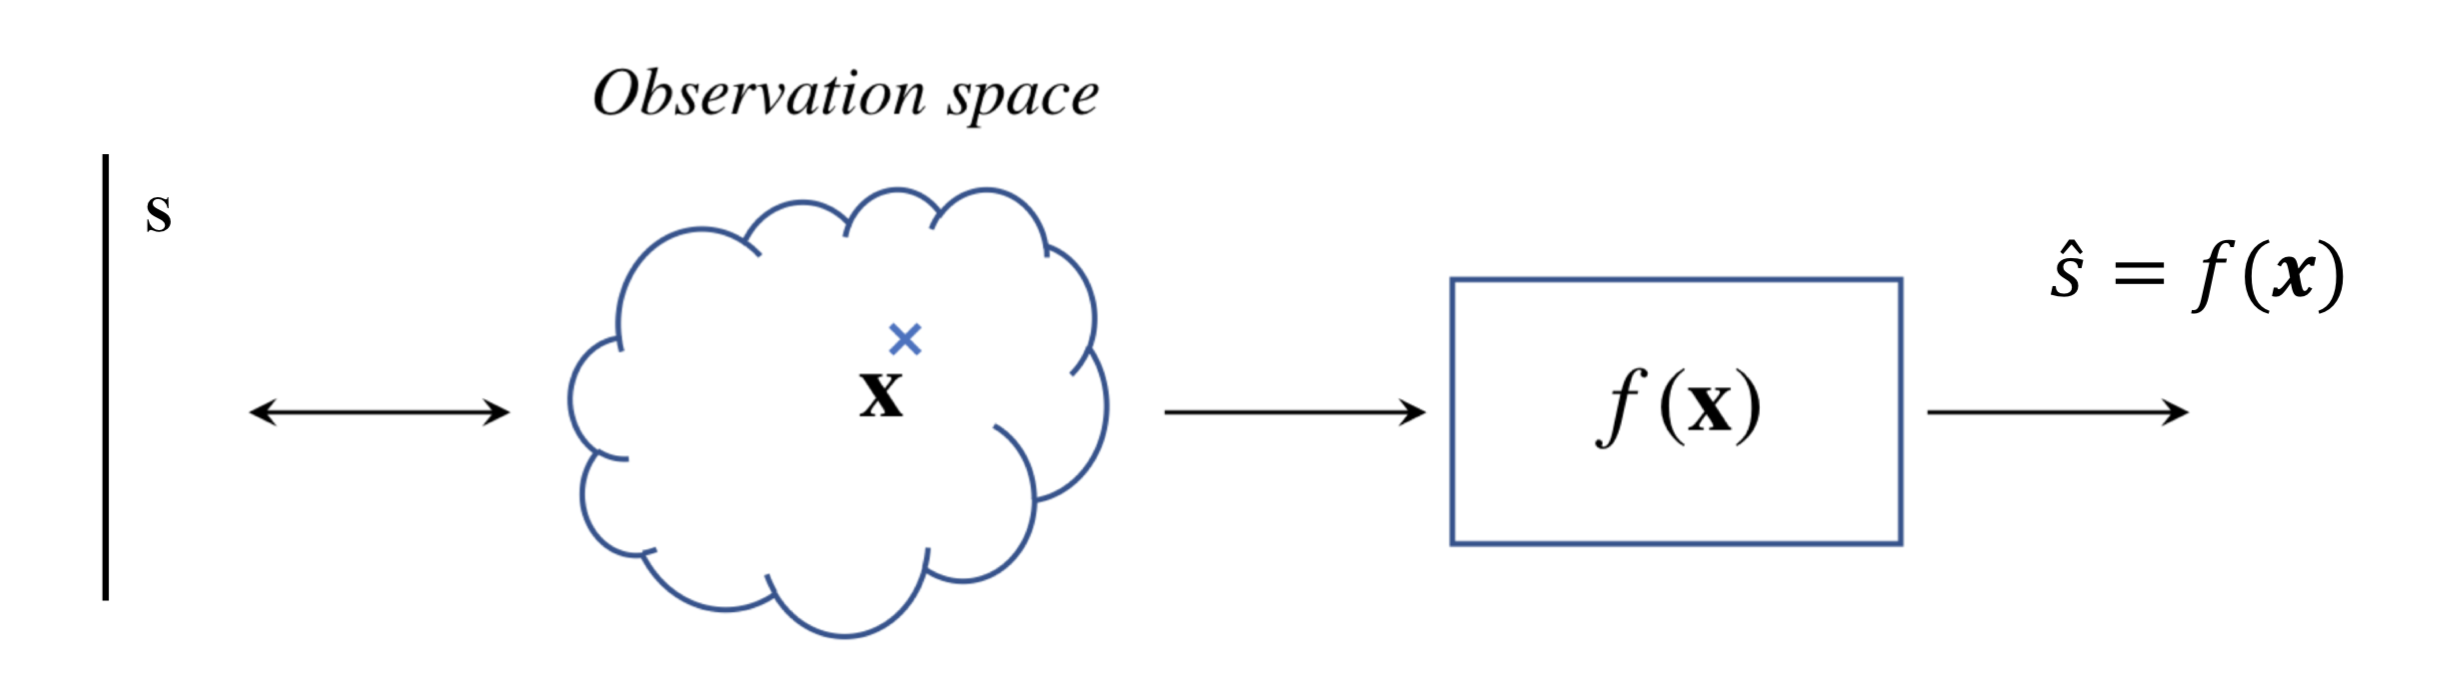
\includegraphics[width=10cm]{Figures//estimation_overview.png}
\end{center}
\caption{Diagram block of estimation problems.\label{fig:est_overview}}
\end{figure}


The estimation module implements a real output function, $\hat{S} = f({\bf X})$, $f(\cdot)$ being the estimation function. It is common to refer to this function simply as {\em estimator}, and to its output as {\em estimation}. A fundamental characteristic of the estimator is the deterministic character of the $f(\cdot)$ function, that is, for a given value $\bf x$ the estimator will always provide the same output. Note that, even though $f(\cdot)$ is deterministic, its output can be modeled as a random variable if we consider the input to the function is random vector $\bf X$.

 Since the estimator is expected to make a certain error in each application, a certain cost  (or, alternatively, a profit) will be entailed. An optimum design of our estimator must take into account this cost during the design minimizing (or maximizing) its mean value.


We consider two different kinds of problems involving estimation problems:
\begin{itemize}
    \item Analysis of estimators: Here, an estimator is given, and our purpose is to analyze its performance with respect to certain performance measure (cost function).
    \item Design of estimators: The goal is to build a function $f(\bf x)$ to optimize a given objective.
\end{itemize}

\subsection{Statistical information involved in estimation problems}
\label{subsec:statistical_info}

Before approaching the design of the estimators themselves, we collect in this subsection the different probability functions that statistically characterize the existing relationship between observations and the variable to be estimated:

%%%%%%%%%%%%%%%
\begin{itemize}
\item First, the {\bf likelihood} of the  variable $S$ is given by $p_{{\bf X}|S}({\bf x}|s)$, and statistically characterizes the generation of observations for each specific value of the variable to be estimated.
\item {\bf Posterior distribution} of $S$: $p_{S|{\bf X}}(s|{\bf x})$. It indicates which $S$ values are more or less likely to concentrate for each particular value in the observation vector.
%In the case where the variable to be estimated is deterministic, it does not make sense to condition the probability distribution of the observations to the value of $s$, so the strictly correct thing would be to denote the probability density of the observations simply as $p_{\bf X}({\bf x})$. However, note that for the estimation problem to make sense, the probability density of ${\bf X}$ has to be different depending on the real value of the deterministic parameter. For this reason, we will sometimes abuse notation and denote that dependence on observations with $s$ as $p_{{\bf X}|s}({\bf x}|s)$, referring to that probability density as the plausibility of $s$.
\item {\bf Marginal or a priori} distribution of $S$: $p_S(s)$
\item {\bf Joint distribution} of ${\bf X}$ and $S$: $p_{{\bf X},S}({\bf x},s) = p_{{\bf X}|S}({\bf x}|s) p_S(s)$. It provides the most complete statistical modeling of the joint behavior of $\bf X$ and $S$.

\end{itemize} 

%%%%%%%%%%%%%

It is important to note that the information available for estimator design may be different in each specific situation. A typical situation, because it is related to the physical process of generating the observations, is the one in which likelihood and the marginal distribution of $S$ are available. Note that from them the calculation of the joint distribution is immediate and the posterior distribution $p_{S|{\bf X}}(s|{\bf x})$ can be calculated by means of Bayes' Theorem. Remember that Bayes' Theorem allows us to obtain the posterior distribution from the {\em a priori} distribution of $S$ and its likelihood:
\begin{equation}
p_{S|{\bf X}}(s|{\bf x}) = \frac{p_{{\bf X},S}({\bf x},s)} {p_{\bf X}({\bf x})} = \frac{p_{{\bf X}|S}({\bf x}|s) p_S(s)}{\int p_{{\bf X}|S}({\bf x}|s) p_S(s) ds}
\end{equation}


\subsection{Cost functions for estimation problems}
\label{subsec_funcion_coste}


The evaluation and design of an estimator requires some objective criteria. In our case, we will consider that this criterion can materialize in the form of some function whose value we seek to maximize or minimize. %We note, however, that there are design strategies that fall outside of this approach, such as the direct maximization of some probability function.

Given that the cost function is associated with a penalty whose origin is in the discrepancy between the actual and the estimated value of $S$, it is common to accept that $c(s,\hat s) \geq 0$, verifying equality when $s = \hat s$. Alternatively, a profit function can be defined whose average value is to be maximized. In addition, it is frequent that the cost function does not depend on the specific values of $s$ and $\hat s$, but on the estimation error that is defined as the difference between the two, $e = s - \hat s$, in which case we have $c(s,\hat s) = c(s - \hat s) = c(e)$.

As an example, some frequently used cost functions are:
\begin{itemize}
\item Quadratic cost: $c(e) = e^2$.
\item Absolute value of the error: $c(e) = |e|$.
\item Relative quadratic error: $c(s,\hat s) = \frac{(s-\hat{s})^2}{s^2}$
\item Crossed Entropy: $c(s,\hat s) = - s \ln \hat s - (1-s) \ln (1-\hat s)$, for $s,\hat{s}\in [0,1]$
\end{itemize}

Accepting that this function\footnote{Note that the cost function is denoted with a $c$ minuscule because it is a deterministic function, i.e., for fixed values of $s$ and $\hat s$ the cost always takes the same value. However, as with the estimation function, the application of that function to random variables will result in another random variable, i.e., $C = c(S,\hat S)$.}  is $c(S,\hat S)$, the evaluation of an estimator is carried out by evaluating the mean value of this cost and the estimator design criterion usually involves the minimization of its mean value; i.e, this cost is used in a statistical sense, evaluating/minimizing its mean value, which is equivalent to evaluating/minimizing the average cost that would be obtained by performing an infinitely large number of experiments.

In general, the mean cost of an estimator is given by
\begin{align}
\label{Est:coste_medio_gen}
\mathbb{E}\{c(S,\hat S)\} 
    & = \int_{\bf x} \int_s c(s,\hat s) p_{S,{\bf X}}(s,{\bf x}) ds d{\bf x}
\end{align}
where it should be noted that $\hat{s}$ is generally a function of ${\bf x}$.




{
%%%%%%%%%%%%%%%
\begin{example}[Evaluation of estimators 1]
\label{CalculoECM}
Suppose that the joint distribution of $S$ and $X$ is given by
\begin{equation}
p_{S,X}(s,x) = \left[
\begin{array}{ll}
\frac{1}{x}, & \qquad 0<s<x ~~{\rm and}~0<x<1 \\
0,           & \qquad \text{otherwise}
\end{array}
\right.
\end{equation}
Let's consider two estimators $\hat{S}_1 = \frac{1}{2}X$ and $\hat{S}_2 = X$. \textquestiondown Which is the best estimator from the point of view of the quadratic cost? To find out, we'll calculate the mean quadratic error for both estimators.
Knowing that, for any $w$,
\begin{align}
\mathbb{E}\{(S-wX)^2\}   
 &= \int_0^1 \int_0^x (s-wx)^2 p_{S,X}(s,x) ds dx   \nonumber\\
 &= \int_0^1 \int_0^x (s-wx)^2 \frac{1}{x}ds dx   \nonumber\\
 &= \int_0^1 \left(\frac{1}{3} - w  + w^2 \right) x^2 dx  \nonumber\\
 &= \frac{1}{3}\left(\frac{1}{3} - w  + w^2 \right) 
\end{align}
Taking $w=1/2$ results in
\begin{align}
\mathbb{E}\{(S-\hat{S}_1)^2\} & = \mathbb{E}\{(S-\frac{1}{2}X)^2\}   
 = \frac{1}{3}\left(\frac{1}{3} - \frac{1}{2}  + \frac{1}{4} \right) = \frac{1}{36}
\end{align}
Alternatively, by taking $w=1$ we get
\begin{align}
\mathbb{E}\{(S-\hat{S}_2)^2\} & = \mathbb{E}\{(S-X)^2\}   
 = \frac{1}{3}\left(\frac{1}{3} - 1  + 1 \right) = \frac{1}{9}
\end{align}
Therefore, from the point of view of the quadratic mean error, $\hat{S}_1$ is a better estimator than $\hat{S}_2$.
\end{example}\vspace{0.4cm}}
%%%%%%%%%%%%%


\begin{example}[Evaluation of estimators 2]
Consider that $X$ is a noisy observation of $S$, so that
\begin{equation}
X = S + R
\end{equation}

where $S$ is a random variable of mean 0 and variance 1, and $R$ is a random Gaussian variable, independent of $S$, of mean $0$ variance $v$. Considering the estimator $\hat{S} = X$, obtain the associated  mean quadratic cost and mean absolute error.

The mean quadratic cost is given by:

\begin{equation}
\mathbb{E}\{(S-\hat{S})^2\} = \mathbb{E}\{(S-X)^2\} = \mathbb{E}\{R^2\} = v
\end{equation}
And the mean absolute error
\begin{align}
\mathbb{E}\{|S-\hat{S}|\}
    &= \mathbb{E}\{|R|\} 
     = \int_{-\infty}^{\infty} |r| \frac{1}{\sqrt{2\pi v}}\exp\left(-\frac{r^2}{2v}\right)dr 
\nonumber\\
    &= 2 \int_{0}^{\infty} r \frac{1}{\sqrt{2\pi v}}\exp\left(-\frac{r^2}{2v}\right)dr 
     = \sqrt{\frac{2v}{\pi}}
\end{align}
\end{example}\vspace{0.4cm}